
%(BEGIN_QUESTION)
% Copyright 2011, Tony R. Kuphaldt, released under the Creative Commons Attribution License (v 1.0)
% This means you may do almost anything with this work of mine, so long as you give me proper credit

Two valves control the flow of methane fuel gas and steam into a reforming furnace, where the two compounds will chemically react to form carbon dioxide and hydrogen gas:

$$\includegraphics[width=15.5cm]{i01693x01.eps}$$

Choose the proper {\it fail-safe mode} for each valve so that there will be nothing but steam inside the catalyst-filled tubes in the event of a general compressed air failure (i.e. both valves losing air pressure).

\vskip 10pt

Steam valve must fail ({\it open} or {\it closed}?) \hskip 100pt Methane valve must fail ({\it open} or {\it closed}?)

\vskip 10pt

Then, determine the proper control action for each controller, assuming both flow transmitters are direct-acting (greater flow = greater output signal to controller).

\vskip 10pt

Steam flow controller action = {\it direct} or {\it reverse}?

\vskip 10pt

Methane flow controller action = {\it direct} or {\it reverse}?

\underbar{file i01693}
%(END_QUESTION)





%(BEGIN_ANSWER)

{\it 2 points for each correct valve failure mode; 3 points for each correct controller action:}

\vskip 10pt

Steam valve must fail \underbar{\bf open} \hskip 100pt Methane valve must fail \underbar{\bf closed}

\vskip 10pt

Steam flow controller action = {\bf direct}

\vskip 10pt

Methane flow controller action = {\bf reverse}

%(END_ANSWER)





%(BEGIN_NOTES)

{\bf This question is intended for exams only and not worksheets!}.

%(END_NOTES)


